\documentclass[14pt]{article}
\usepackage{graphicx}
\usepackage{hyperref}

\title{Tugas 2 Robust Control : Uncertainty }
\author{Donny Prakarsa Utama\\ \texttt{3332170032}
\and Ringga Dwi Raju\\ \texttt{3332170029} }
\maketitle

\begin{document}
For the following uncertain systems, obtain a weight obtain a weight $W(s)$ so that the uncertain systems are approximated by those with multiplicative dynamic uncertainty. Compare gain plots of the original and obtained uncertain models. (Use ureal.m & ultidyn.m. Read User’s guide of Robust Control Toolbox, Ch. 6.)\\
1. $G(s)=\frac{1}{s+1}e^{-\theta s} ,\theta \in [0,0.1]$\\

Jawab :
Uncertainty pada soal ini hanya ada pada delay $ \theta $, dan dapat dibentuk menjadi $G(s)=\frac{e^{-\theta s}}{s+1}$ maka ditulis pada MATLAB
\begin{verbatim}
    exptheta =  ureal('exptheta',1.0526,'PlusMinus',[-0.0526,0.0526]);
\end{verbatim}
Kemudian buat fungsi alih nya menjadi
\begin{verbatim}
    sys = tf(exptheta ,[1 1])
\end{verbatim}
Untuk pembobotan manual $W(s)$ didapat
\begin{verbatim}
    W = tf([1],[0.8 0.8]) 
\end{verbatim}\\
Pembobotan menggunakan fungsi makeweight didapat
\begin{verbatim}
    W1 = makeweight(1.2,0.67 ,0)
    bodemag(sys, 'b' , sys.NominalValue ,'g', W, 'k', W1, 'r')
\end{verbatim}
Hasil dari bodeplot ada di Figure 1
\begin{figure}[h]
    \centering
    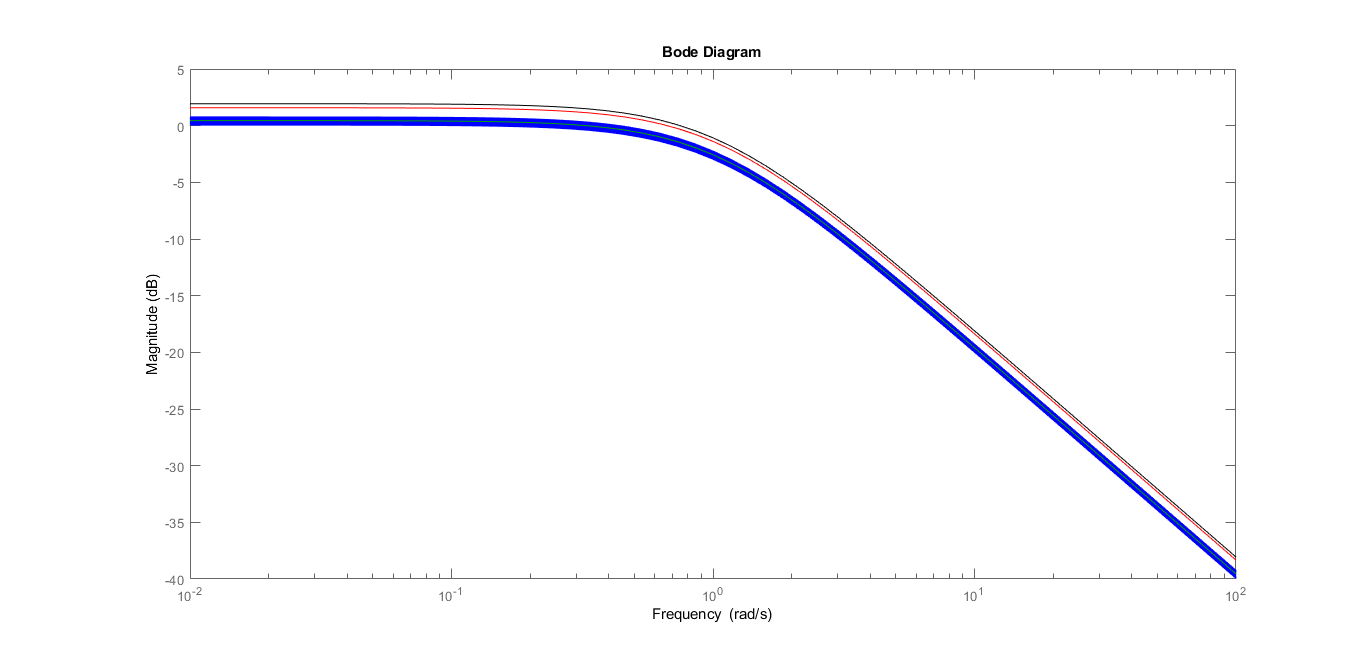
\includegraphics[width=90mm]{makeweight1.png}
    \caption{$W(s)$ manual(hitam) dan makeweight(merah) \label{overflow}}
\end{figure}\\
2. $G(s)=\frac{1}{T_{1}s+1}.\frac{1}{T_{2}s+1} ,T_{1} \in [0,0.2], T_{2} \in [2,2.5]$ \\

Jawab : ada 2 Uncertainty yaitu $T_{Slow}$ dan $T_{Fast}$, dan fungsi alih dapat dibentuk menjadi $ \frac{1}{T_{1}T{2}s^2 + (T_{1}+T_{2})s + 1}$ karena $\omega(s)\Delta(s)=\frac{G(s)}{G_{o}(s)}-1$ dapat dibuat "norm" pada listing MATLAB
\begin{verbatim}
    t1 = ureal('t1', 0.1, 'PlusMinus',[-0.1,0.1]);
    t2 = ureal('t2', 2.25 ,'PlusMinus',[-0.25,0.25]);
    sys = tf([1],[t1*t2 t1+t2 1])
    sys0 = tf([1],[t1.NominalValue*t2.NominalValue t1.NominalValue+t2.NominalValue 1])
    norm=sys/sys0 - 1
\end{verbatim}\\
Untuk pembobotan manual $W(s)$ didapat
\begin{verbatim}
    W = tf([-0.7 -0.6 0.02],[1/28 -1 1])
\end{verbatim}\\
Pembobotan menggunakan fungsi makeweight didapat
\begin{verbatim}
    W2= makeweight(0,2,28);
    bodemag(norm, 'b', W2,'r')
\end{verbatim}
Hasil dari bodeplot ada di Figure 2
\begin{figure}[h]
    \centering
    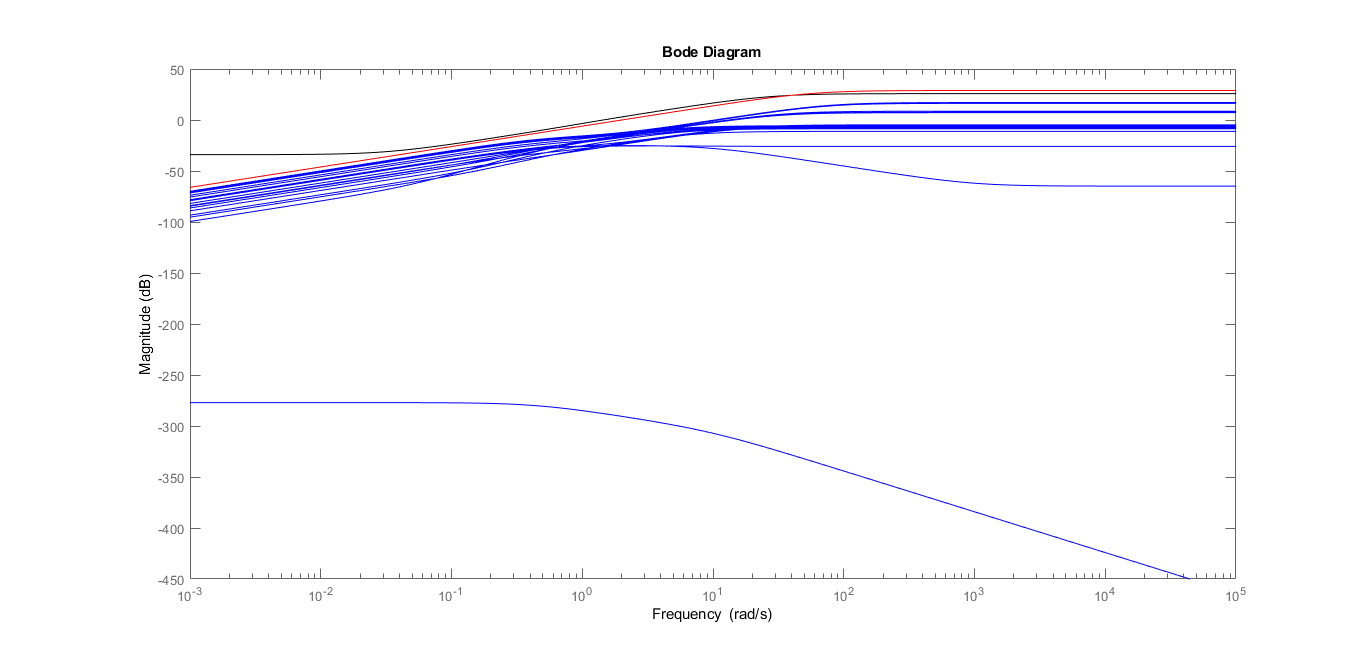
\includegraphics[width=90mm]{makeweight2.png}
    \caption{$W(s)$ manual(hitam) dan makeweight(merah) \label{overflow}}
\end{figure}\\
3. $G(s)=\frac{1}{s+1}.\frac{\omega^2}{s^2+2\zeta\omega s+\omega^2},\zeta \in [0.1,0.2],\omega\in[90,110]$\\

Jawab : ada 2 uncertainty yaitu $\zeta$ dan $\omega$ fungsi alih dapat dibentuk menjadi $   \frac{\omega ^2}{s^3+(2 \zeta   \omega +1)s^2+(2 \zeta   \omega + \omega ^2)s+\omega ^2} $
\begin{verbatim}
    w = ureal ('w', 100, 'PlusMinus',[-10,10]);
    z = ureal ('z',0.15 , 'PlusMinus',[-0.05,0.05]);
    sys= tf([w^2],[1 2*z*w+1 2*z*w+w^2 w^2])
    sys0= tf([w.NominalValue^2],[1 2*z.NominalValue*w.NominalValue+1 2*z.NominalValue*w.NominalValue+w.NominalValue^2 w.NominalValue^2])
    norm=sys/sys0 - 1
\end{verbatim}
% Untuk pembobotan manual $W(s)$ didapat
% \begin{verbatim}
%     W = tf([1],[0.8 0.8]) 
% \end{verbatim}\\
Pembobotan menggunakan fungsi makeweight didapat
\begin{verbatim}
    W3= makeweight(0,102,-5);
    bodemag(norm, 'b' , W3 ,'r')
\end{verbatim}
Hasil dari bodeplot ada di Figure 3
\begin{figure}[h]
    \centering
    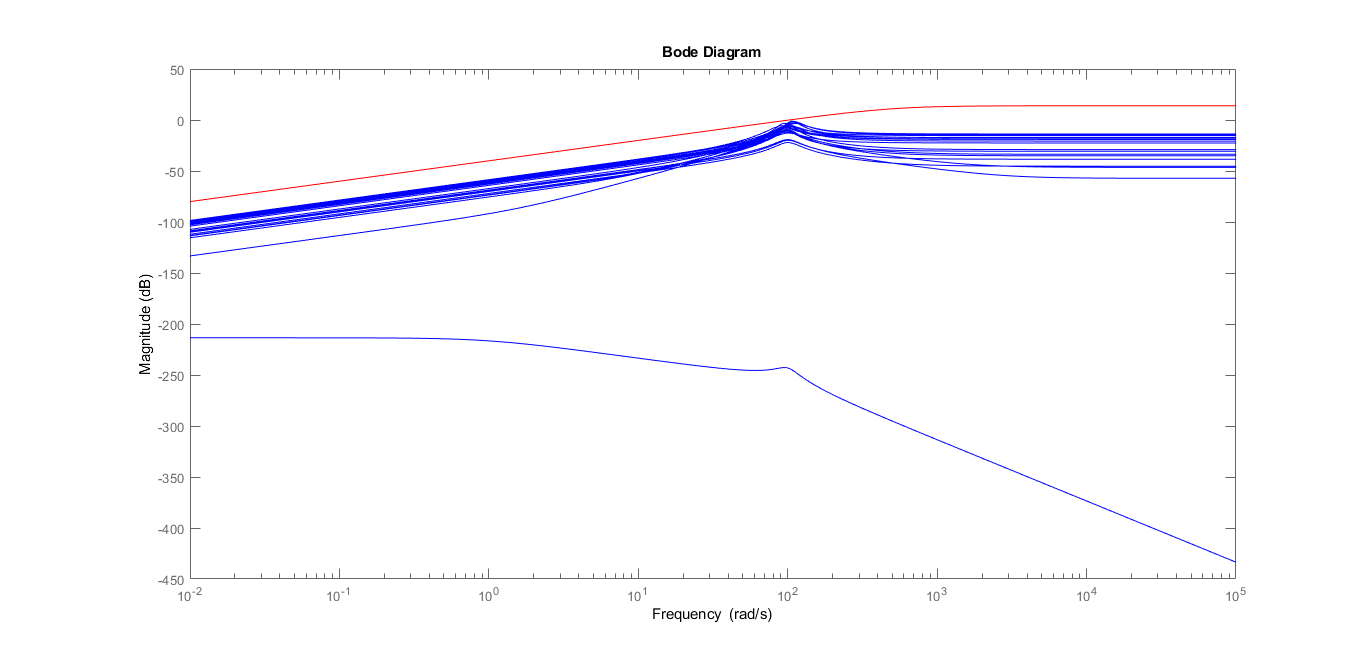
\includegraphics[width=90mm]{makeweight3.png}
    \caption{$W(s)$ makeweight(merah) \label{overflow}}
\end{figure}\\

Full Code on  Github :

Matlab : \href{https://github.com/utamadonny/matlabcolle/blob/master/KendaliNew/uncertainty.m}{uncertainty.m}

LaTex Build : \href{https://github.com/utamadonny/BelajarLatex/blob/master/Robust2/Robust2.tex}{Robust2.tex}
\end{document}

